% Intended LaTeX compiler: pdflatex
\documentclass[ppgc,english]{iiufrgs}

\usepackage{tabularx}
\usepackage{hyperref}
\usepackage[utf8]{inputenc}
\usepackage{booktabs}
\usepackage{enumitem}
\usepackage[T1]{fontenc}
\usepackage[linesnumbered,ruled,boxed,commentsnumbered]{algorithm2e}
\usepackage{listings}
\author{Barros de Assis}{Lucas}
\advisor[Prof.~Dr.]{Mello Schnorr}{Lucas}
\def\titlepagespecificinfo{Introduction to High-Performance Computing}
\def\manualleg[#1]{{\centering\legend{#1}\par}}
\renewcommand{\nominataCoord}{Prof.~Alberto Egon Schaeffer Filho}
\renewcommand{\nominataCoordname}{Coordenador do PPGC}
\keyword{x}
\translatedkeyword{x}
\translatedtitle{x}
\date{Agosto}{2024}
\title{Analysing the CPU's influence on GPU equipped nodes}
\hypersetup{
 pdfauthor={Lucas Barros de Assis},
 pdftitle={Analysing the CPU's influence on GPU equipped nodes},
 pdfkeywords={},
 pdfsubject={},
 pdfcreator={Emacs 28.2 (Org mode 9.5.5)}, 
 pdflang={English}}
\begin{document}

\maketitle

\chapter{Introduction}
\label{sec:org4420b40}

Heterogeneous architectures seem to be the default configuration for clusters dealing with HPC. Hardware accelerators such as
GPUs achieve parallelism levels way beyond those attainable by general computing cores, and dense linear algebra libraries such
as Chameleon \cite{chameleon} provide kernels to extract maximum performance on such architectures.

Although the CPU is absolutely necessary no matter the programming model being used, when dealing with task-based runtime systems
such as StarPU \cite{starpu}, capable of exploiting such powerful accelerators on top of the conventional cores, its influence on the
total computation time can be questioned.

Kestur et al. \cite{kestur} compared a matrix-vector multiplication on CPU, GPU and FPGA and
found a better performance on a parallel CPU implementation. However, due to their FPGA limitations, this work was limited to small
matrices (around 65536 elements) that could not profit from all the power available. Xiong and Xu \cite{xiong} did similar comparisons
with the matrix multiplication operation and bigger matrices. Their study shows that the difference in performance increases with
the matrix size, and for their biggest matrices the GPU implementation took about 20\% of the duration of the CPU implementation.

In this study, we used the LU factorization implementation from the Chameleon library to compare two nodes with the same GPU but different
CPUs in hope of providing some insight on the matter. We used matrices bigger than the ones employed on the previously cited works and
added both Intel's Hyper-threading technology and i9's P-cores and E-cores architecture into the equation.

\chapter{Materials and Methods}
\label{sec:org4bcf267}
The experiments were run on the \emph{tupi} machines, part of the cluster maintained by the \emph{UFRGS} university.
The nodes \emph{tupi1} and \emph{tupi2} have each an \emph{Intel Xeon E5-2620 v4} and nodes \emph{tupi3} and \emph{tupi4} are each equipped with
an \emph{Intel Core i9-14900KF}. Each of these nodes has also a \emph{GeForce RTX 4090}, but the \emph{Xeon} equipped nodes use
\emph{PCI-e 3.0} while the \emph{i9} use \emph{PCI-e 4.0}.

We used the spack \cite{spack} application to control the software stack, allowing it to be compiled
for each CPU's own microarchitecture - \emph{Broadwell} on the \emph{Xeon} and \emph{Skylake} on the \emph{i9}. We used the StarPU runtime
system on commit 146ce9d8 and the Chameleon library on commit 3e958439.

\emph{StarPU} creates performance models for the available hardware during its runs, which allows it to properly apply its scheduling techniques.
Each configuration was repeated 6 times and had its worst performance removed to mitigate the effects of the calibration performed.
The resulting graphs were drawn by plotting the average time of each configuration and its standard deviation.

\section{Input data}
\label{sec:org74a54f5}

The Chameleon library provides testing binaries used for both numerical verification of its methods and performance analysis. In this study,
we employed these binaries to execute the LU factorisation of single precision matrices with sizes 65,536x65,536 and 100,000x100,000.

The execution parameters were the matrix size, the tile's block size, the amount of CPU and GPU workers and the existence of a \emph{CUDA} exclusive
core when using GPU. Each configuration was repeated 5 times on shuffled scripts, trying to scatter the execution of same configuration runs.
All of the matrices were created by Chameleon's matrix generation algorithm with the same seed.

\section{CPU-only experiments}
\label{sec:orge779b40}

As a starting point, we ran experiments without employing the GPUs computational power, which proved to be an opportunity to take a look at
their individual performance.

\emph{Intel}'s \emph{Hyper-threading} technology consists in using one single physical core to run the threads assigned to a
second virtual core. This technique aims to make better use of the superscalar hardware to dispatch more than one instruction simultaneously.
In this case, however, the \emph{Hyper-threaded} cores share the same available memory between the pair, instead of each one having its own cache.

The \emph{Intel Core i9} CPU has 24 cores separated in two categories: Performance-cores (\emph{P-cores}) and Eficient-cores (\emph{E-cores}). While the
P-cores are larger, capable of \emph{Hyper-threading} and designed for raw speed, the E-cores are smaller and designed to maximize efficiency \cite{intel-hybrid}.

When working with the runtime system \emph{StarPU}, we need to define a strategy for the scheduler to assign the tasks to the available hardware. The
CPU-only experiments employed the \emph{dmda} strategy, meaning that the tasks are scheduled as soon as they become available to the core where their
termination time will be minimal taking in account the transfer time.

\section{Tupi experiments}
\label{sec:orga63fa3b}

Adding the GPUs to the pool of available resources allowed us to actually check the CPU's influence on the full node's performance. When working with
\emph{CUDA}, \emph{StarPU}'s configuration let us determine which thread will perform the \emph{CUDA} operations and if it will work exclusively on these instructions or it will
receive its share of tasks. This option added a new variation for the experiments, that were run both with a \emph{CUDA} exclusive thread and without it. The \emph{i9}'s
runs with this dedicated thread had it always on one of its P-cores.

Another modification was the scheduling strategy that was changed to the \emph{dmdas}, similar to the \emph{dmda} employed on the CPU-only experiments except it sorts the
available tasks by priority.

After running the first experiments on the full nodes, we realized the GPU was not using all of its memory, so new experiments were added with 100,000x100,000
matrices, achieving around 90\% of the \emph{GeForce RTX 4090} available memory.

\chapter{Results}
\label{sec:orgc7e57ac}

As expected, Figure \ref{fig:org8e3b083} shows the \emph{i9}'s performance is considerably better than the \emph{Xeon}'s. Regarding the \emph{Hyper-threading}, it appears to
improves both CPU's performance as long as we use small enough blocks. The simultaneous multithreading technique stops being worth it when
their blocks get big enough to need memory from outside their caches.

\begin{figure}[htbp]
\centering
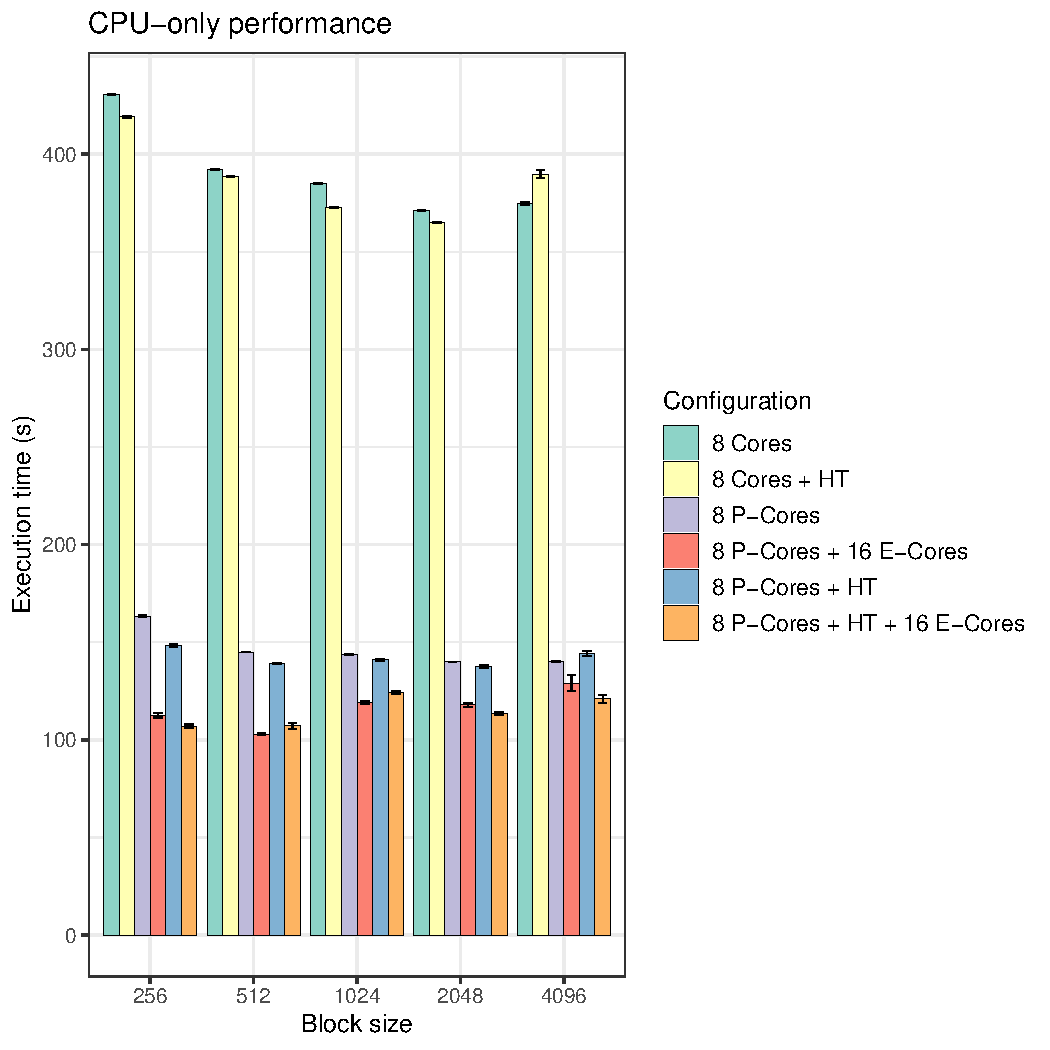
\includegraphics[width=.9\linewidth]{./figures/cpu_only.pdf}
\caption{\label{fig:org8e3b083}Comparison between the CPU-only experiments}
\end{figure}

Adding the \emph{i9}'s E-cores brought some variability to the performance. This is probably explained by the fact that \emph{StarPU}'s performance models
considered both P-cores and E-cores as computing unities with the same capabilities.

When looking at the execution times of each CPU's best experiment, the \emph{i9} performs around 3.64 times faster than the \emph{Xeon}.

The performance analysed with the GPUs available is shown in Figure \ref{fig:org89d910c}. The first aspect to observe is that the experiments
with a \emph{CUDA} dedicated core performed better than the ones without it.

\begin{figure}[htbp]
\centering
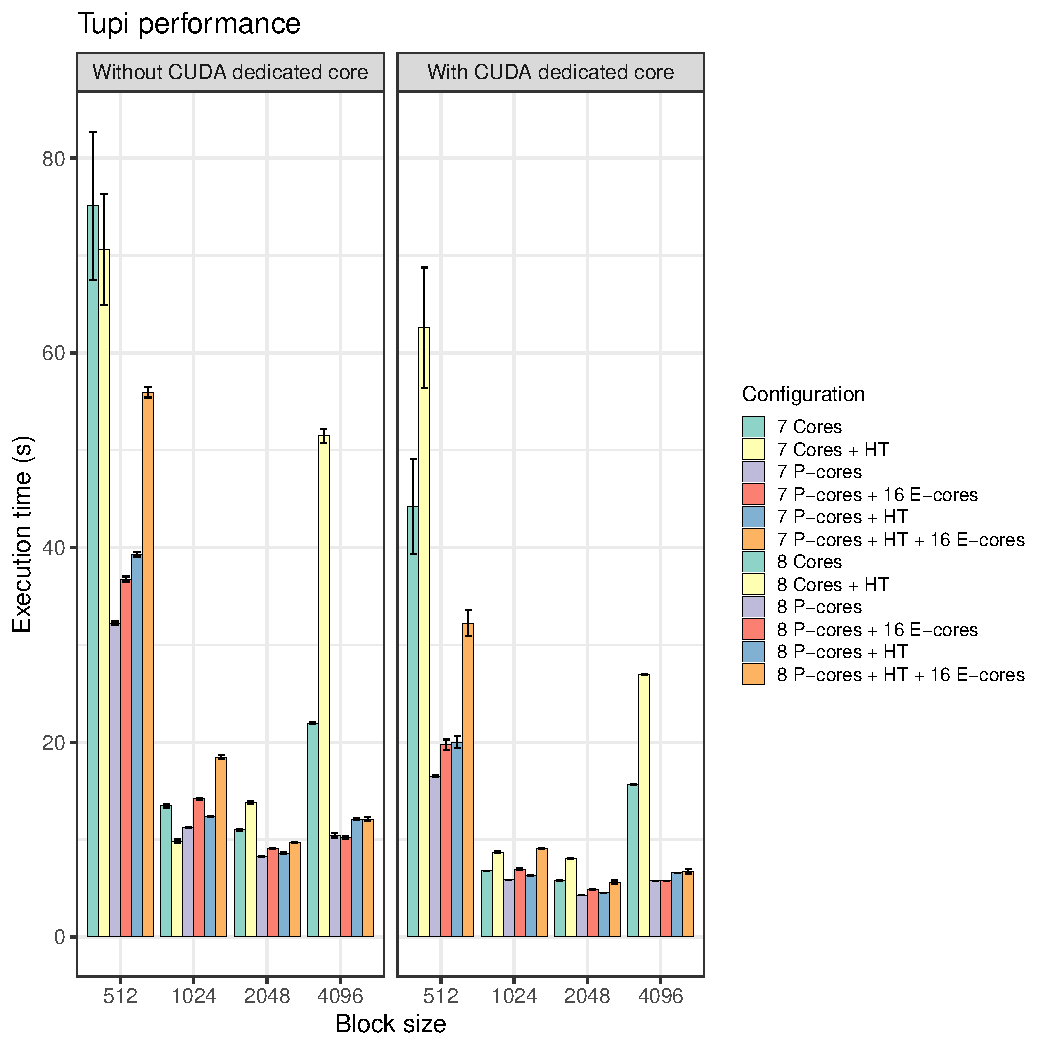
\includegraphics[width=.9\linewidth]{./figures/tupi.pdf}
\caption{\label{fig:org89d910c}Comparison between the full node experiments}
\end{figure}

When there is no exclusive \emph{CUDA} thread the \emph{Xeon} nodes once again profited from the \emph{Hyper-threading} technology as long as their block
sizes were small enough. However, the \emph{i9}'s performance seems to be always negatively affected by both the \emph{Hyper-threading} and the
addition of E-cores. One possible explanation is once again the performance models not properly adapted to such different workers.

Including a thread for the \emph{CUDA} operations we can see the same behavior on both \emph{Xeon} and \emph{i9}, extracting the best performance when
there are no logical nor efficient cores involved.

While using only the CPU the \emph{i9}'s best case was around 3.64 times faster than \emph{Xeon}'s. When the GPUs were added, this difference
decreased to around 1.34 times, which shows that the employ of accelerators reduce the significance of the CPU's capacities.

Figure \ref{fig:org88de64e} shows the results when achieving 90\% of the GPU's memory usage. In this case, the \emph{Hyper-threading} technique decreased
the performance even with small blocks on the \emph{Xeon} without a dedicated \emph{CUDA} core, possibly because of the bigger amount of \emph{CUDA} operations
to be performed on larger matrices. Other than that, the E-cores seemed to slightly increase the performance, which could indicate that
their extra memory cache compensates for the performance model's issues.

Finally, by exploiting more of the GPU's memory, the speed ratio between the \emph{Xeon} and the \emph{i9} CPUs increased to around 1.77, reinforcing
the hypothesis that an increase on the amount of \emph{CUDA} operations requires more from the CPU.

\begin{figure}[htbp]
\centering
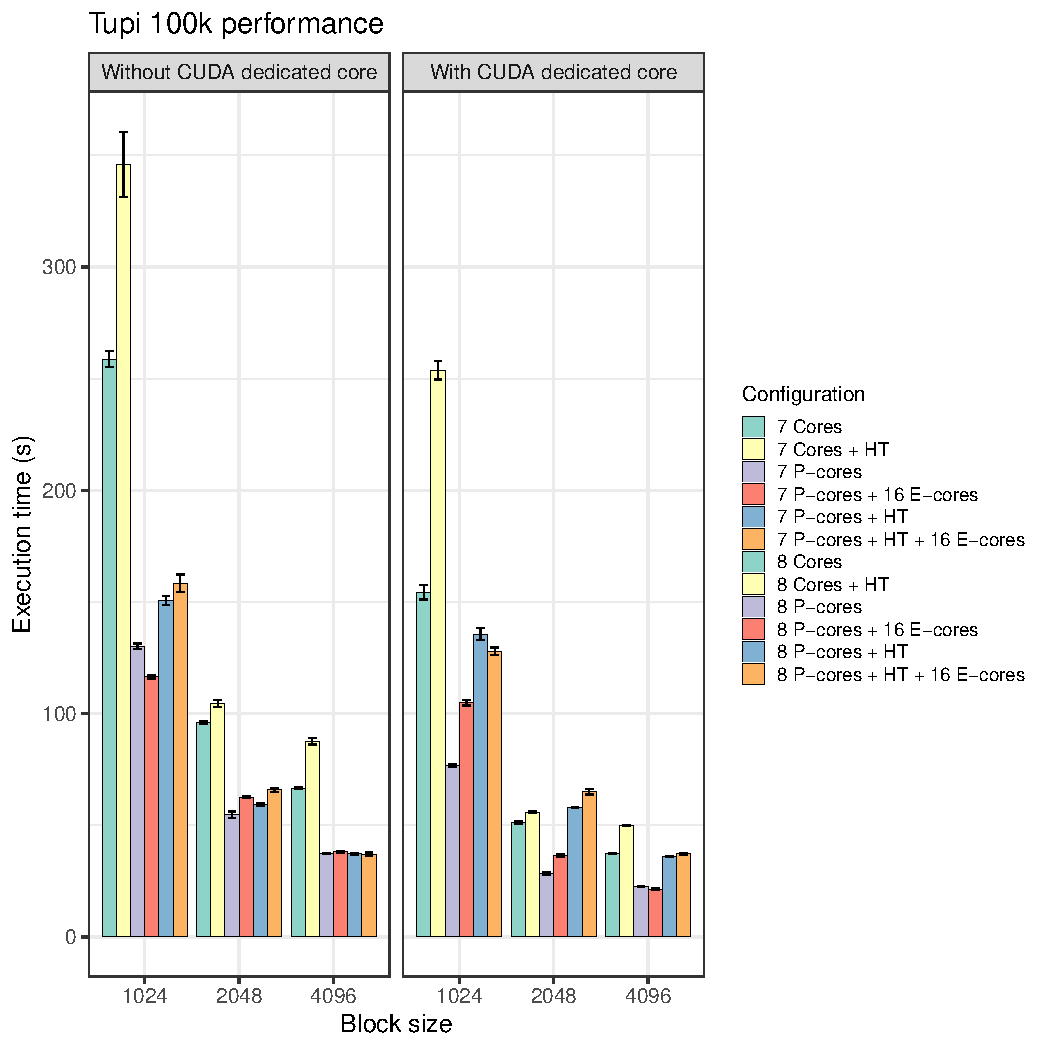
\includegraphics[width=.9\linewidth]{./figures/tupi_100k.pdf}
\caption{\label{fig:org88de64e}Comparison between the full node experiments with 100kx100k matrices}
\end{figure}


\chapter{Conclusion}
\label{sec:orgcd5b1d6}

In this study, we verified the CPU's influence when working with parallel dense linear algebra operations assisted by
GPUs. We compared the performances when employing \emph{Intel}'s \emph{Hyper-threading} and P-cores/E-cores technologies with and without
the accelerators involved. Even though the accelerators presence decreased the performance difference between the CPUs studied,
the gap was increased when we exploited better the GPU's memory, suggesting that larger GPUs require faster CPUs.

\section{Future Works}
\label{sec:org229f6b4}

By studying the \emph{i9} CPU, we realized that the \emph{Hybrid design} concept of having performance and efficient cores can be further
analysed in order to extract all of the potential it may have. Trying to differentiate their behavior with the runtime system
is a possible way of doing this, as well as employing them as \emph{CUDA} dedicated cores to check their performance at it.


\bibliographystyle{abntex2-alf}
\bibliography{refs.bib}
\end{document}